\section{Introduction}
% \textcolor{orange}{Structure
% \begin{enumerate}
%     \item detail the users' need for personalization -- scenarios and tasks
%     \item state the challenges of current personalized chatbots to motivate our research questions
%     \item highlights of our data: entire conversation history over a wide variety of tasks, closely surrounding personas. concatenation enables scalable generation
%     \item list the evaluation tasks
%     \item results preview
%     \item list of contributions
% \end{enumerate}}

In recent years, Large Language Models (LLMs) have rapidly evolved as general task solvers, demonstrating remarkable performance \citep{srivastava2023beyond,zhou2023instruction,yue2024mmmu,rein2024gpqa}. 
% As these models mature, 
Today, many users rely on LLMs as their \textit{personalized} chatbots or assistants in a wide range of daily tasks -- from offering writing support \citep{mysore-etal-2024-pearl,tian-etal-2024-large-language} to delivering recommendations \citep{hua2023tutorial} or consultations \citep{xie2024travelplanner, zheng2024natural}, etc. Personalization in LLMs involves adapting model responses to specific traits, preferences, and historical interactions of each user, moving beyond generic responses to more relevant and tailored ones. Since different users have different personas, it becomes an emergent need for LLMs to be \emph{pluralistic}—capable of adapting to different user characteristics across different scenarios~\citep{sorensen2024position, jiang2024peek, xie2024wildfiregpt, kirk2024prism}, thereby enhancing user experience and engagement. 

% To provide personalized responses, LLMs face a practical challenge: they often cannot easily access to all information about the user. 
For LLMs to deliver personalized responses, a practical challenge lies in the fact that LLMs cannot easily access all the information about a user. 
This challenge is further amplified by the \textit{ever-changing} nature of user preferences over time \citep{radlinski2017theoretical, dean2022preference}. For example, as illustrated in Figure \ref{fig:overview}, a user initially said, \textit{"I like pizza"}, but mentioned in a later session, \textit{"I've started exploring gluten-free options,"} upon discovering a gluten allergy. 
% Following multiple interactions on unrelated topics, 
When the user again asks for food recommendations, a personalized LLM chatbot should be able to track the change, and provide recommendations according to the user's current situation. Current LLM chatbots often fail to recognize and adapt to evolving user personas. This may lead users to perceive these chatbots as less helpful and empathetic, ultimately diminishing satisfaction~\citep{aggarwal2023artificial, ait2023power}. 
% in LLM-based chatbots 

%If the chatbot recommend some cuisine based on the incorrect recall of user's preference or not show any understanding of users, user would perceive the interaction with the chatbots not that engaging and helpful. This level of dynamic personalization significantly enhances user-centric interactions, fostering empathy and engagement, key factors in advancing AI chatbot development \citep{aggarwal2023artificial, ait2023power}. key factors in advancing AI chatbot development \citep{aggarwal2023artificial, ait2023power}.

In this work, we evaluate LLMs' ability to leverage the \textit{past interaction history} with a user in order to deliver a personalized response in real time. Recent studies \citep{lin-etal-2024-interpretable, shi2024wildfeedback, zhao2025prefeval} have found that user-LLM interactions can be a rich (but often implicit) information source on the user's characteristics and preferences.
However, it remains an open question whether LLMs can effectively use the interaction histories to (1) internalize the user’s inherent traits and preferences, (2) track how the user's characteristics evolve over time, and (3) generate personalized responses accordingly in new scenarios.

%%% Original
% To study these questions, we propose the \datasetnameemoji~benchmark, which features over 180 simulated user-LLM interaction histories, each with up to 60 multi-turn conversation sessions across 15 personalized task scenarios. We construct \datasetname~by first curating a high-quality set of user profiles with detailed persona information, where each user's characteristics change over time with events happening in their life. 
% Based on the state of a user profile at a given point in time, we simulate conversation sessions, where the user seeks personalized suggestions from LLM within one of the personalized tasks scenarios, such as travel planning, therapy consultation or food recommendation, etc. We assemble a user's complete interaction history with LLM, by concatenating the conversation sessions in temporal order, so that the evolution in the user profile over time is reflected in the history.  

To study these questions, we propose the \datasetnameemoji~benchmark, comprising over 180 simulated user-LLM interaction histories with up to 60 multi-turn sessions across 15 personalized task scenarios. Each history is built from a detailed user persona whose characteristics evolve over time. Based on the user's profile at different points, we simulate task-specific conversations (e.g., travel, therapy, food) and concatenate them in temporal order to capture the user’s profile evolution throughout the entire interaction history.



% We curate detailed user profiles that surround diverse personas sampled from a large persona database \citep{ge2024scaling}. 
% We then simulate entire conversation histories in which users dynamically reveal changes in their traits and preferences over time. 
% \datasetname~ features over 180 simulated user-LLM interaction histories. Each user profile includes comprehensive data from up to 60 multi-turn conversation sessions and 1$M$ tokens, capturing a diverse range of interactions. 
% These conversations span 15 realistic conversation scenarios specifically chosen to require personalization, such as tailored recommendations, personalized writing assistance, and adaptive consultations. 
% Finally, we introduce fine-grained challenges to evaluate how effectively models can leverage their knowledge of the user to generate personalized content and recommendations across diverse application scenarios.

%We also present fine-grained challenges to assess how effectively the model can utilize its memory about the user to generate personalized content and recommendations in diverse application scenarios.
%[TODO: list our question types]

%By integrating detailed personas with extensive historical data and realistic tasks, \datasetname provides a robust and nuanced framework to systematically evaluate and advance the personalization capabilities of LLMs.
\begin{figure}[t]
  \centering
  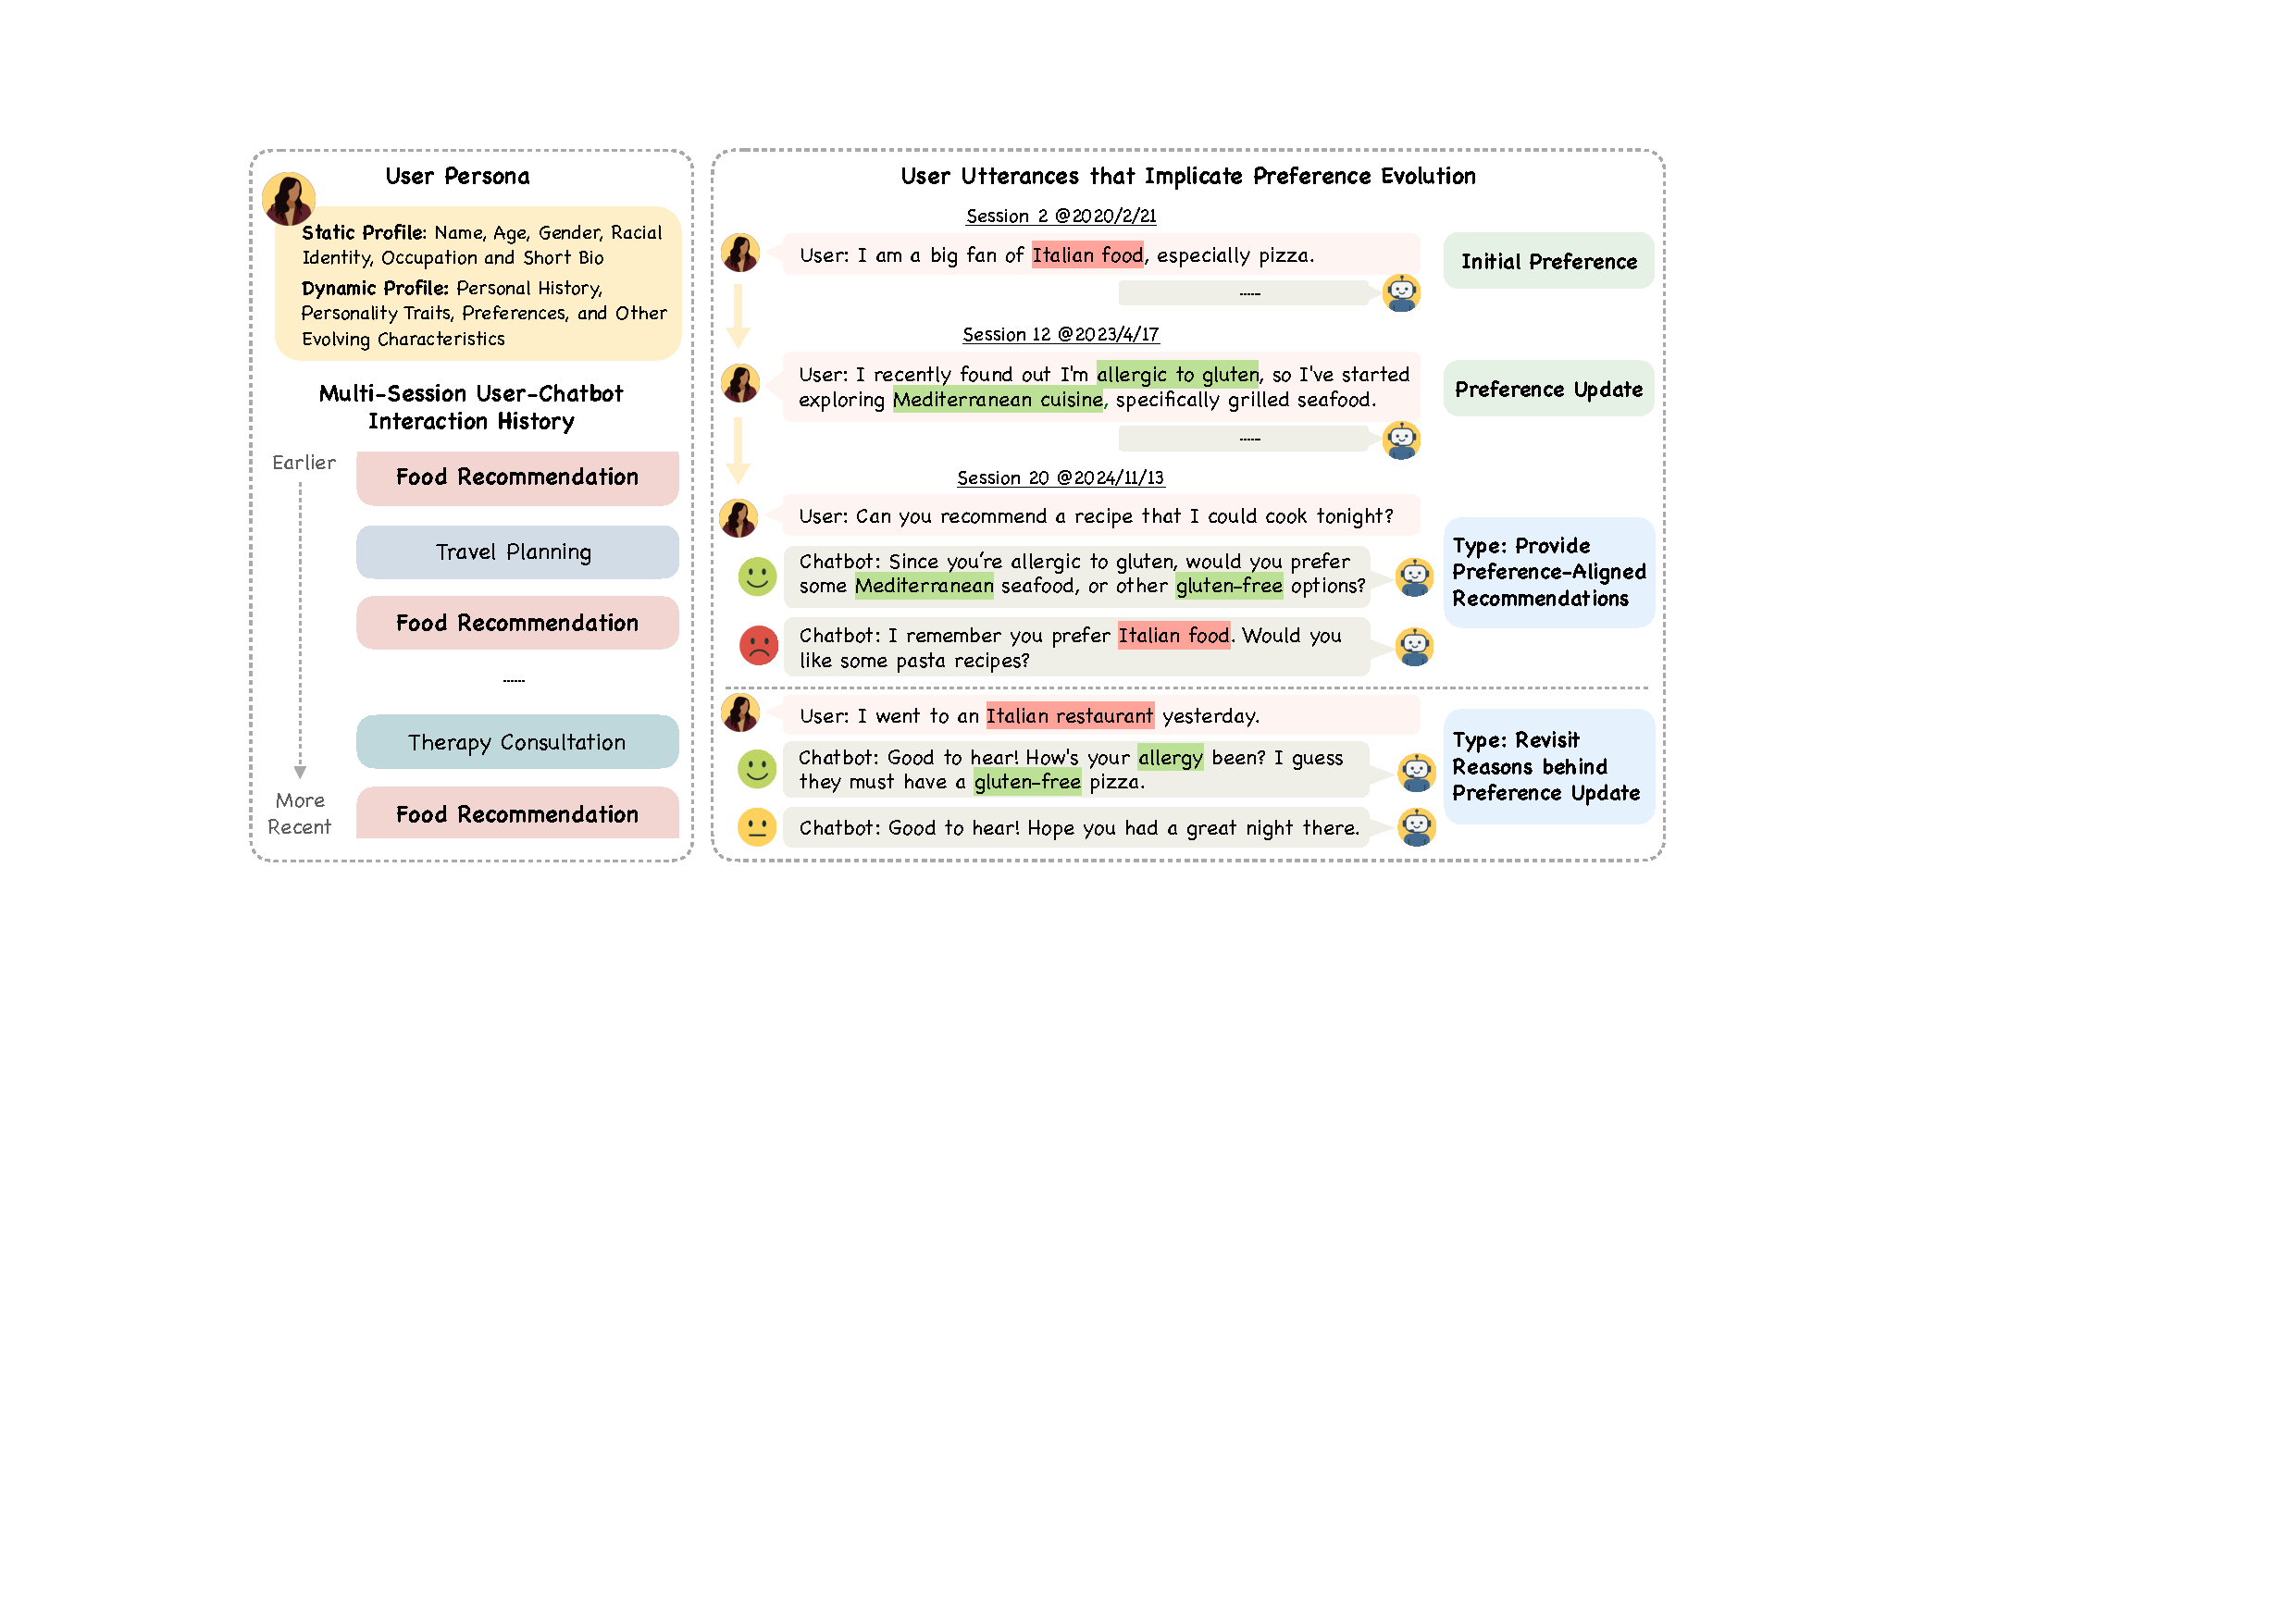
\includegraphics[width=1\linewidth]{figures/bench_overview.pdf}
  \caption{Overview of \datasetname~benchmark. Each benchmark sample is a user persona with static (e.g., demographic info.) and dynamic attributes (e.g., evolving preferences). Users engage with a chatbot in multi-session interactions across a variety of topics such as food recommendation, travel planning, and therapy consultation. As the user's preferences evolve over time, the benchmark offers annotated questions assessing whether models can track and incorporate the changes into their responses.}
  \vspace{-5mm}
  \label{fig:overview}
\end{figure}

%%% Original
% With \datasetnameemoji, we evaluate the ability of state-of-the-art LLMs to infer a user profile and how it evolves over time, as well as whether LLMs can apply what they learn about the user to provide personalized responses in different task scenarios. For this purpose, we design 7 types of \textit{in-situ} user requests (as shown in \autoref{tab:qa_types}), where the user issues new requests to LLM in a new conversation session from the first-person perspective. We evaluate if LLM is able to select the correct response that is aligned with the user's current state among distractor options. Overall, we observe that current LLMs still struggle to provide personalized responses based on the user's profile, with the frontier models such as GPT-4.5, o1, or Gemini-2.0-Flash scoring only around $50\%$ accuracy. 
% While models are typically performing reasonably well on recalling simple facts from the users and recognizing changes in users' preferences (with $60$-$70\%$ accuracy across models), they often struggle on acknowledging users' current situations, and delivering personalized responses accordingly (with $30$-$50\%$ accuracy). We provide detailed analysis on the factors that may impact model performance, such as the length of the interaction history, position in which the user preference is first/last mentioned, as well as the effect of having a separate retrieval component for memory recall, etc.  

With \datasetnameemoji, we evaluate whether state-of-the-art LLMs can infer evolving user profiles and generate personalized responses across task scenarios. To emulate the realistic settings in user-LLM interactions, we design 7 types of \textit{in-situ} user queries (\autoref{tab:qa_types}), where users issue queries to LLMs from first-person perspectives. We evaluate whether LLMs can select the correct response that best aligns with the current state of the user. We find that frontier models such as GPT-4.1, o4-mini, GPT-4.5, o1, or Gemini-2.0-Flash score only around $50\%$ overall accuracy and Llama-4-Maverick slightly lower at $43\%$ using direct prompt approaches.
While models perform reasonably well on recalling facts and tracking preference changes (60–70\% accuracy), they struggle to incorporate users’ latest situations into responses (30–50\% accuracy). We provide detailed analysis on how factors such as history length, preference positioning, and memory components may impact performance.

% We observe that current LLMs still struggle to recognize the dynamic evolution in users' profiles over time through direct prompt approaches.
% As a consequence,  LLMs often fail to deliver responses that align with users' current situations and preferences. We hope that \datasetname, along with our proposed user profile and conversation simulation pipeline can facilitate future research in the development of truly user-aware chatbots.

To summarize our key contributions and findings:
\begin{itemize}[itemsep=2pt, left=0pt]
\vspace{-2mm}
\item We propose the \datasetnameemoji~benchmark and its synthetic dialog generation pipeline for persona-oriented, multi-session, and timelined user-chatbot interaction history. 
% to evaluate LLMs capability to deliver personalized response across 15 task scenarios. 
% Our benchmark concerns realistic user-centric settings. We ground data generation on diverse user personas, closely reflecting real-world conversation scenarios that require personalization capabilities.
\item We assess 15 LLMs on 7 types of \textit{in-situ} user queries and evaluate their ability to provide responses aligned with user's dynamically changing profile across 15 task scenarios.    
% We develop a cost-effective, flexible, and scalable approach for generating synthetic conversation data tailored to multi-turn user-model interactions.
% \vspace{2mm}
\item With \datasetname, we observe that frontier models such as GPT4.1, o4-mini, GPT-4.5, o1, DeepSeek-R1, Gemini-2.0, Llama-4, and Claude-3.7 still struggle to be user-aware and deliver personalized responses, especially when the knowledge of the user needs to be applied across new scenarios. 
% with the biggest challenge in delivering personalized responses in new scenarios.
% responses according to user's latest preference and situation, and reason over users' profiles across different task scenarios.  
% Frontier models such GPT-4.5 and Gemini-1.5 achieve the highest personalization performance but still hover around only 52\% accuracy in multiple-choice settings, while reasoning models such as o1, o3-mini, and DeepSeek-R1 also struggle with the task. Generalization to new scenarios remains the greatest challenge in personalization.
% \item 
\end{itemize}
% in order for our data to achieve this goal. what data look like: simulated user profile and across different scenarios (list all), interact over time-->reflect their changes of xxx and be draw from session interaction.

% In practice, however, a practical difficulty comes from the fact that LLMs do not readily have access to all information about an user.  

% they are increasingly being deployed as personalized assistants, offering recommendations, consultations, and context-aware responses that adapt to individual user needs.

% Many users today rely on LLMs as their \textit{personalized} chatbots for a wide range of tasks. They harness these models’ assistance in everything from everyday planning to specialized problem-solving [TODO: add scenarios from papers].
% As these models become ever more ubiquitous in daily workflows, their ability to adapt to individual user profiles and preferences has grown in significance for enhancing user satisfaction and trust. Yet, achieving robust personalization at scale introduces several challenges, including accurately representing user profiles derived from extensive conversational histories and effectively tracking their continuous evolution over time. 

% For example, as illustrated in Figure\ref{fig:overview}, a user previously interacting with an LLM chatbot for food recommendations explicitly stated, "Following classic recipes is a better choice than experimenting with fusions," and elaborated her reasoning. Even after moving on to other unrelated tasks, the user's subsequent interactions continue to expand her historical profile. Therefore, the next time she seeks food recommendations, a well-personalized LLM should align its suggestions with the user's established preference for traditional cuisine or acknowledge her perspective explicitly. In contrast, poorly personalized responses might inaccurately recall user preferences or fail to capture the evolving nature of her interests over time [TODO: give examples of out incorrect answers]. Such challenges highlight the critical need for systematic benchmarking to ensure LLMs consistently "know" users deeply and "respond" effectively throughout ongoing interactions.

% In this work, we introduce the \datasetname~ benchmark to assess personalization performance across three key aspects:
% [TODO: callout our three questions]
% \begin{enumerate}
%     \item Can LLMs accurately learn about users' inherent traits and preferences from extensive interaction histories?
%     \item Can LLMs effectively track and recognize how users' preferences and situations evolve over time?
%     \item  Can LLMs use what it knows about the user to adapt their responses accordingly?
% \end{enumerate}


% Memory is a fundamental capability for enabling Large Language Models (LLMs) to act as agents~\citep{kapoor2024ai, jiang2024towards, durante2024agent}, capable of adapting to diverse user personas~\citep{ge2024scaling} and preferences in dynamic, interactive, and conversational scenarios. By maintaining a good memory of prior interactions, a model can develop long-term, personalized engagements with user's preferences, background, and context. Without a memory, it could make responses that merely make sense in general, or fail to adapt effectively to each user's unique needs. Therefore, proper handling of memory serves as a cornerstone towards personalization~\citep{chen2024persona, zhang2024personalization, chen2024large}, allowing LLMs to tailor their outputs based on previous interactions with users, enhancing user satisfaction.

% Although numerous research advances have been made to enhance and investigate the memorization capabilities of LLMs, a comprehensive benchmark suite that rigorously evaluates their \textit{memory recall in personalized scenarios} is still lacking. Most existing memory benchmarks are constrained only to contrived, relatively simple factual recall tasks \cite{liu2024lost}, lacking the complex user personas and long-term contextual nuances essential for genuinely personalized interactions \citep{maharana2024evaluating, wu2024longmemeval}.
% % TODO: tencent

% Unlike existing long-term memory benchmarks, we aim to evaluate whether LLMs can recall user personas and preferences over prolonged user-agent conversations, moving beyond static knowledge to dynamic updates across sessions at different times. We also present fine-grained challenges to assess how effectively the model can utilize its memory about the user to generate personalized content and recommendations in diverse application scenarios.
% To summarize our contributions:
% \begin{itemize}[noitemsep]
% \item Our benchmark concerns realistic user-centric settings. We ground data generation on diverse user personas, closely reflecting real-world conversation scenarios that require memory capabilities.
% \item We extend the evaluation of memorization to personalized generation, utilizing memory to generate persona-oriented conversations across diverse topics.
% \item We develop a cost-effective, flexible, and scalable approach for generating synthetic conversation data tailored to long, multi-turn, and multi-session user-model interactions.
% \end{itemize}

% TODO: One of the contributions is to simulate realistic scenarios of users using AI models as assistants. We can define what realistic means in our work. 


